\chaptermark{An essay on transsportation}
% Renmoved form old housing Chapter, which was  included in Extensions.
{\color{red}
\section{An essay on transportation costs and the city}
One of the first applications of the model was to the effect of a transportation revolution. The advent of first rail transportation and then the automobile radically changed the size, productivity, and population distribution of cities.
periphery available, allowing larger lot sizes and larger homes for those who can afford them.

\begin{figure}[!hb]
\centering
% CHANGING TRANSPORTATION COSTS
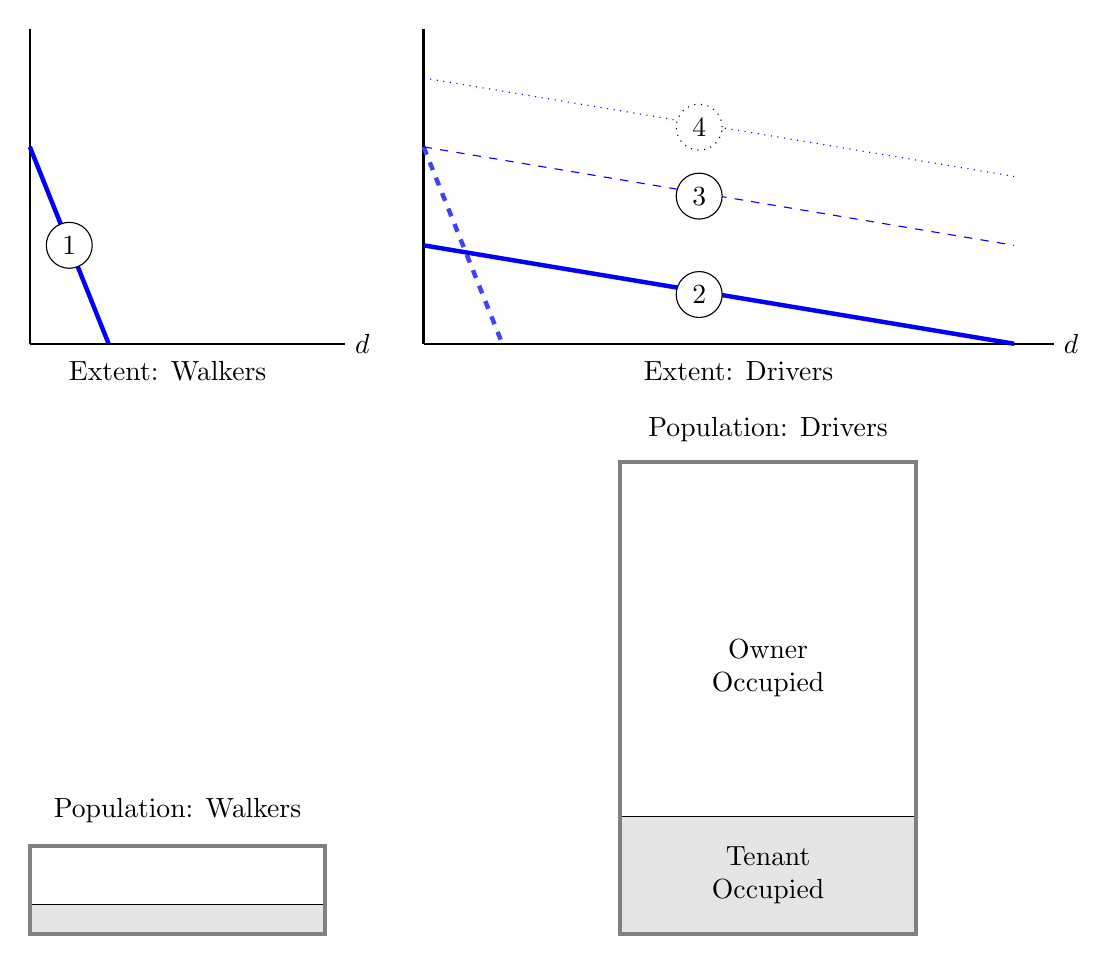
\begin{tikzpicture}[scale=.5]
% EXTENT  BEFORE
\draw[thick](0,0)--(0,8); %Y
\draw[thick](0,0)--(8,0)node[right]{$d$};
\node at (3.5,-.7){Extent: Walkers};
\draw[ultra thick, blue](0,5)--(2,0); 
\node[circle,draw=black, fill=white, inner sep=3pt,minimum size=10pt] (b) at (1,2.5) {1};

% POPULATION BEFORE
\begin{scope}[shift={(0, -15cm)},scale=1.5]%population
\draw [fill=gray!20,] (0,0) rectangle (5,.5); 
\draw[line width= .5mm, black!50] (0,0) rectangle (5,1.5);
\node at (2.5,2.1){Population: Walkers};
\end{scope}

% EXTENT AFTER
\begin{scope}[shift={(10cm, 0)}]
\draw[thick](0,0)--(0,8); %Y
\draw[thick](0,0)--(16,0)node[right]{$d$}; %X
\node at (8,-.7){Extent: Drivers};
\draw[ultra thick, blue!75, dashed](0,5)--(2,0);
\draw[ultra thick, blue](0,2.5)--(15,0);

\node[circle,draw=black, fill=white, inner sep=3pt,minimum size=10pt] (b) at (7,1.25) {2};

\draw[ blue, dashed](0,5)--(15,2.5);
\node[circle,draw=black, fill=white, inner sep=3pt,minimum size=10pt] (b) at (7,3.75) {3};

\draw[ blue, dotted](0,6.75)--(15,4.25);
\node[circle,draw=black, dotted,fill=white, inner sep=3pt,minimum size=10pt] (b) at (7,5.5) {4};
\end{scope}

% POPULATION AFTER
\begin{scope}[shift={(15, -15cm)},scale=1.5]%population
\draw [fill=gray!20,] (0,0) rectangle (5,2); 
\draw[line width= .5mm, black!50] (0,0) rectangle (5,8);
\node at (2.5,8.55){Population: Drivers};
\node at (2.5,4.5)
    [text width=2.4cm, align=center]
    {\baselineskip=20pt Owner Occupied};
%\node at (2,3.3)    [text width=2.4cm]    {\baselineskip=20pt Mortgaged};
\node at (2.5,1)
    [text width=2.4cm, align=center]
    {\baselineskip=20pt Tenant Occupied};
\end{scope}
\label{fig-rent-driving}
\end{tikzpicture}
\caption{Housing tenure post transportation revolution.}
\label{fig-transport-tenure}
\end{figure} 
 
%\input{fig_TransportCost.tex}

The transportation cost revolution brought about by the first street cars and later automobiles made much larger cities possible.  The average walking pace is 2.5 to 4 mph, and new transportation technologies raise this rate by a factor of between five and ten, increasing potential urban area by between twenty-five and one hundred times. 




% THIS IS INTERSTING K.  morgages: Effect of a finbancial instument on urban form!!  suburban flight, second half of the century

%Electric trolleys drew upon manufacturing technology that appeared only in the eighteen eighties and at first only in America. 

%As with other transportation revolutions, institutional as well as technological revolutions were necessary for the interurban phenomenon to succeed.  One such institutional revolution was the creation of the home mortgage in the eighteen eighties.  Another was the development of the public utility, a regulated monopoly, in the earlier twentieth. century.\footnote{https://faculty.washington.edu/jbs/itrans/charge20.htm} The automotive revolution was as important in its way as the coming of the railroads.

%The automobile in time established even more powerful synergies, but they weren't present at the beginning.  Roads suitable for automobiles scarcely existed though new methods of paving utilizing macadam or concrete had recently been invented.  Furthermore, there was no good model in place for road construction.   Unlike the case with either light or heavy rail systems, the vehicles and the road itself were not part of the same corporate entity.       

%Once automotive ownership assumed certain proportions toward the close of the teens of the century, the automobile began to transform the landscape of America in an even more fundamental way than the streetcars had. 

%From the second decade of the twentieth century, the automobile in America has been linked with suburban flight, and when the growth of suburbs reached a crescendo early in the second half of the century, automobile ownership became the norm. 

% Because exurbs are already numerous and growing more so, they place considerable pressure on the Body Politic to ensure that fuel prices remain low, for if prices rise beyond a certain point the exurbanites will be forced to sell out, probably at ruinously low returns because few will choose to live in isolated areas without affordable transportation.  True, exurbs could conceivably be served by public transportation, but only at enormous cost per rider because the population densities are so low in the areas where they are located \dots

% That places the vast suburb dwelling public at risk and the exurbanites most of all.

Initially, rents fell at the centre and rose outside of the original city limits. Lower rents and cheaper suburban housing attract more workers, so that central rents and the land values they support  rise to the original levels and then, because the rising population makes the
city more productive, beyond the original level. 

It  also affected social structure and left indelible marks on the form of cities developing at the time and after. In North America, with large amounts of land, it generated massive urban sprawl, but also made land available for a growing `middle class' of homeowners. This homeowning middle class became the dominant social formation in North 
American society. 

Ultimately the urban expansion generated congestion and rising transportation cost that began to limit urban growth, put upward pressure on  housing costs including transportation, and therefore downward pressure on middle-class effective incomes. Rising congestion costs steepen the rent profile and  reduce the net productivity of cities. Although the process is not a focus of this thesis it represents a relatively simple extension for later work.

\subsection{Differential transportation costs}
 Urbanists agree that before the railroad and the automobile, the extent of a city was roughly determined by how far a person could walk in about an hour. The time and effort cost of transportation determined the size of cities. 
 
 It also affected the distribution of the classes within the city. When everyone walked, the  wealthy may have valued their time more than the poor. In terms of the model, the willingness to pay of the rich would higher  near the core than  the willingness (or ability) to pay of  the poor, but would descend more rapidly with distance
\begin{figure}
\begin{center}
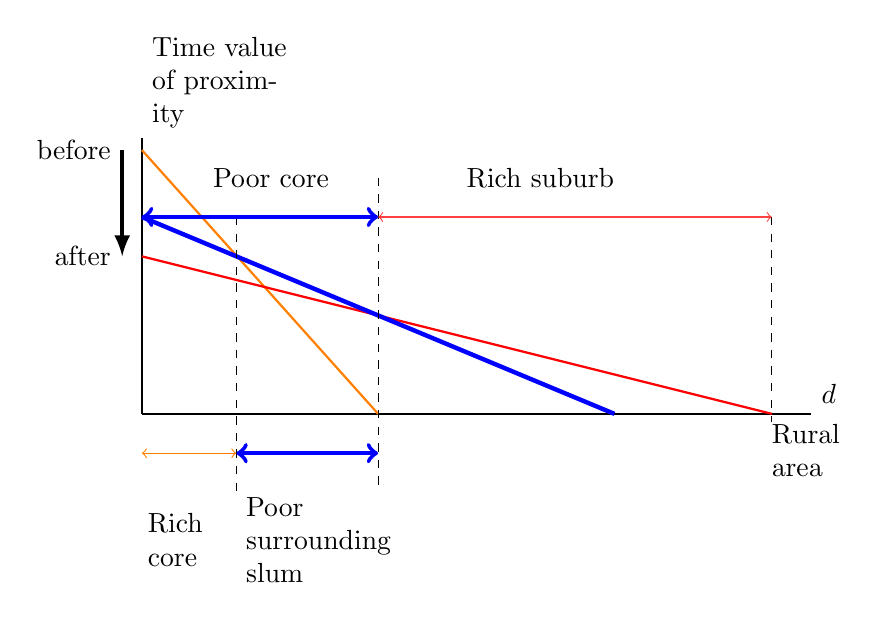
\begin{tikzpicture}[scale=1]
% AXES
\draw[thick](0,0)--(0,3.5)node[above right, text width=1.8cm]{Time  value of proximity}; %Y++
\draw[thick](0,0)--(8.5,0)node[above right]{$d$}node[below, text width =1cm]{Rural area}; 
% BIDS-RENT CURVES
\draw[thick, orange](0,3.35)--(3,0);
\draw[thick, red](0,2)--(8,0);
\draw[ultra thick, blue](0,2.5)--(6,0);

\draw[-latex, ultra thick](-.25,3.35)node[left]{before}--(-.25,2)node[left]{after};
% ZONE DIVISIONS VERTICAL LINES
\draw[dashed](1.2,2.5)--(1.2,-1) ;
\draw[dashed](3,3)--(3,-1) ;
\node at (4,3)[right]{Rich suburb};
\node at (2.5,3)[left]{Poor core};
\draw[dashed](8,2.5)--(8,-.1) ;
%  ARROWS BEFORE
\draw[<->, orange](0,-.5)--(1.2,-.5);
\draw[<->, blue, ultra thick](3,-.5)--(1.2,-.5);
\node[text width =1cm,  left] at (1.2,-1.6){Rich core };
\node[text width =1cm, right] at (1.2,-1.6){Poor \\ surrounding slum};
%  ARROWS AFTER
\draw[<->, blue, ultra thick](0,2.5)--(3,2.5);
\draw[<->, red!75](3,2.5)--(8,2.5);

% \draw[ blue, dashed](0,5)--(15,2.5);
% \node[circle,draw=black, fill=white, inner sep=3pt,minimum size=10pt] (b) at (7,3.75) {3};

% \draw[ blue, dotted](0,6.75)--(15,4.25);
% \node[circle,draw=black, dotted,fill=white, inner sep=3pt,minimum size=10pt] (b) at (7,5.5) {4};
\end{tikzpicture}\end{center}
\caption{A prediction of the basic model: if transportation cost for the rich falls, shifting the orange  bid-rent curve for the rich to the location of the red line, we will see a shift of housing for the rich  from the core to the suburb.}
% \label{fig_fix_my_label}
\end{figure}

 If the technology suddenly provides the rich with commuter trains or automobiles and more attractive sites at the edge of the city, the orange line could drop enough  and become much flatter leading in a flight of the rich to the suburbs, as appears to have happened in many American cities. Lower transportation costs make cheaper land on the edge of the city attractive. This would  offer  more space and the opportunity to build larger homes, a pattern that has emerged in some cities.

\textbf{Experiments}: We first turn off financial  demand and partition the population by wealth and transportation cost to  verify that the predictions made by researchers hold in our model. We then turn financial demand back on  and see if the rate or degree of financialization differs from the base model


\subsection{Municipal costs and revenue}

\begin{figure}
\begin{center}
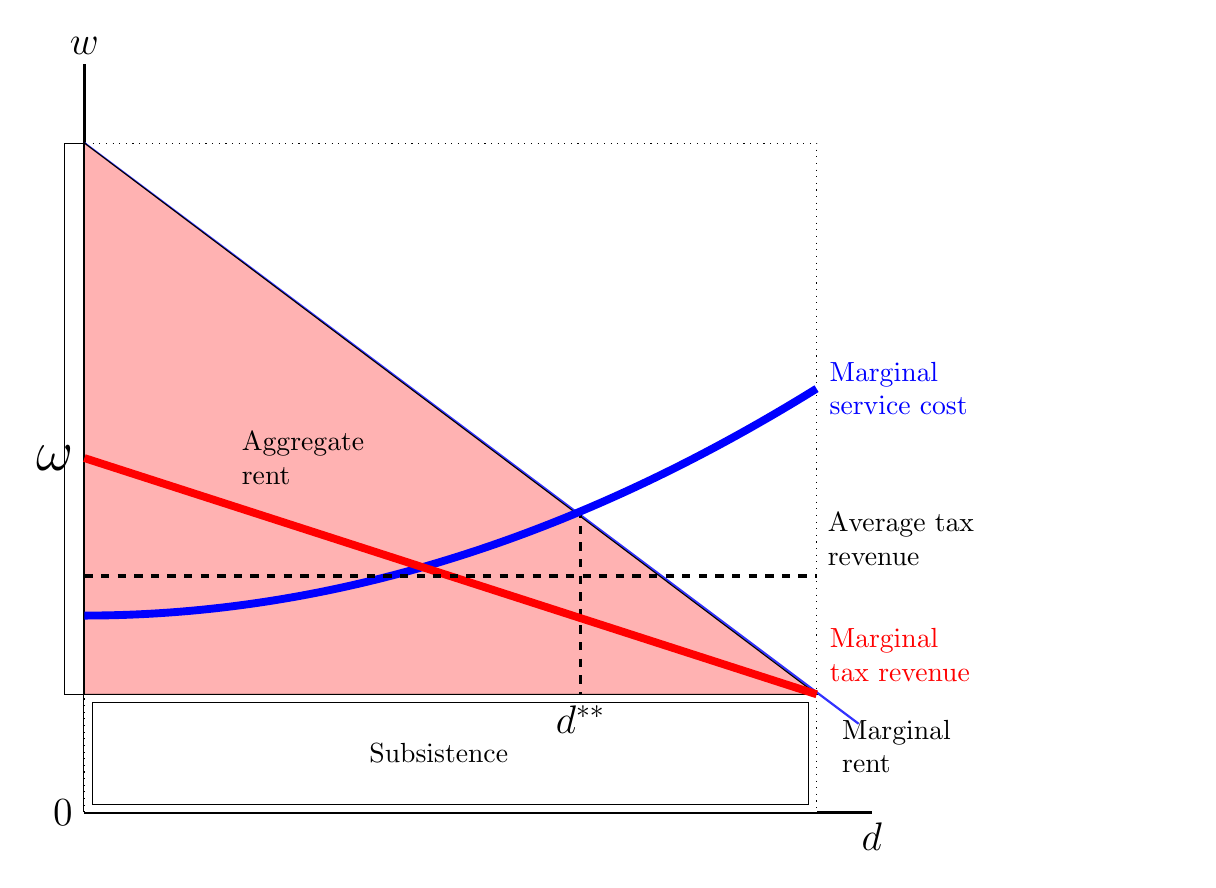
\begin{tikzpicture}[scale=1]
\def\bndmax{5}        %https://tex.stackexchange.com/questions/68462/filling-a-complex-region-with-tikz
\def\bndmin{0.2}
\def \n {8}  % height of y axis
\def \d {10}  % length  of x axis
\def \t {.75}  %  cost of transportation per unit x
\def \th {1}   %
\def \w {7}    %  wage premium
\def \om{1.5}%  omega =rural wage Zero for urban population
\def \azero{2}
\def \aprime {-.0}	
\tikzset{func/.style={thick,color=blue!80}}	
\draw [thick] (0,-\om) --(\d,-\om)node[below]{\Large $d$};  			% Zero for rural population
\draw [thick] (0,-\om)node[left=.5]{\Large $0$} --(0,\n)node[above]{\Large $w$};	% Y axis

%\draw [thick] (0,0)node[left=.5]{ subsistance}--(\d,0);
\node[left=.25] at (0,3){\huge $\omega$};
%\node[left=.25] at (0,\w+.3){subsistence plus};
%\node[left=.25] at (0,\w-.4){wage premium};	

\draw[fill=white, white] (0.1,-0.1) rectangle (14,-\om+.1);
\draw [] (-.25, 0) rectangle(.25, \w);%fill=green!30!blue!30
\node[right] at  (.25, \w/2){Added Productivity};
%\draw [ thick, ->](11.3,-\om/2)--(13, -\om/2)node [right] {\Large $d$};
\draw[fill=blue!40] (0.1,-0.1) rectangle (9.2,-\om+.1);

\draw[fill=black!0, dotted] (0,-\om) rectangle (9.30,\w);% new product repeat
\draw[func, domain=0:\w/\t+.5] plot [samples=200] (\x,{\w-\t*\x}); %rent profile
\draw[fill=blue!0] (0.1,-0.1) rectangle (9.2,-\om+.1);
\node at (4.5,-\om/2){Subsistence};
\draw[fill=red!30,] (0.,0.)--(0,7)--(9.30,0.)--cycle;% Rent \w-.2
\node[text width=2cm] at (3.,3){Aggregate \\rent}; 		%Rent 
%\node at (5.8,5.7)[]{\Large Transportation};
\node at (6.3,4.8)[white]{\Large expenditure};
\draw[ line width=.5mm, dashed] (6.3,2.35)--(6.3,0)node[below ]{\Large $d^{**}$};

\draw[func, domain=0:9.3, line width=1mm,blue, text width=2cm] plot [samples=200] (\x,{1+\x^2/30})node[right]{Marginal\\ service cost};
\draw[ line width=1mm, red] (0,3)--(9.3,0)node[above right, text width=3cm ]{Marginal\\tax revenue};
\node at (9.5, -.2)[below right, text width=2cm]{Marginal rent};

\draw[ line width=.5mm, dashed] (0,1.5)--(9.3,1.5)node[above right, text width=2.5cm ]{Average tax revenue};
%GRID
%\draw[step=1cm,gray,very thin] (0,0) grid (10,10);
\end{tikzpicture}
\end{center}
\caption[The Alonso model with municipal costs and revenue.]{The Alonso model \gls{rent profile}, as illustrated in Figure~\ref{fig-alonso-simple}, with cost and municipal costs and revenue added.} %service fees added.}
\label{fig-municipal-costs}
\end{figure}
 

 Two stylized facts should be noticed. The first is that the marginal cost of servicing generally rises with the distance from the centre. Figure illustrates the general form of servicing costs, but not the relative scales of rent and servicing costs. When this observation is combined with the \gls{Henry George Theorem} the conclusion is that the optimal size of the city  is at  $d^{**}$, where marginal service cost intersects with the marginal increase in total urban rent.  Walter Christaller, 1933

The second stylized fact is that property taxes, which are generally  fixed as a share of property value, decline as the distance from the centre increases. Figure~\ref{fig-municipal-costs} illustrates the general form of tax liabilities, although it does not  accurately represent their relationship to rent or  servicing costs. This implies that in many or most urban situations the residents at the outer edges pay less than the average amount in property tax per unit of land, but cost  the community budget more than the average amount. In essence, the central city subsidizes the suburbs. (see Perverse Cities \ref{blaisPerverseCitiesHidden2011}). This arrangement is both economically inefficient and unfair, but it has been built into the fiscal structure of cities largely as a result of automobile-based urban growth. It is likely that this fiscal misallocation saps some of the potential productivity growth of cities. Property taxation reduces the market value of properties, but it also funds services and amenities that increase the value of properties. 

Both servicing and taxation effects are more variable and than the simple model suggests.  One conclusion urban theorists draw based on variants of the Alonso model is that because property owners in the low-density urban margin are subsidized,  the subsidy is likely to create serious fiscal problems for municipalities in the long-term and result in serious inefficiency in land use.

Political opposition is essentially rent seeking.

}